\section{Goals of the Protocol}
\label{sec:secure-goals}

Recall that when making a payment, the Customer first views the price about to be charged on the screen of the Retailer's Point of Sale.
Using this information, the Customer makes his one and only decision: whether to allow the payment protocol to occur, or not.
The underlying assumption that the Customer makes is that the price displayed on the screen is equal to the price which will be charged to his Credit Card.
This need not be the case: the information displayed on a screen is merely an assurance in the informal sense:
	the numbers displayed to the customer \emph{should} reflect the dollar amount which will subsequently be sent with the Charge Request message to the bank,
    but there is no mechanism in place to require this.
Two attacks emerge as a result.
The goal of the Secure CC Protocol presented in this chapter is to extend the protection provided by the Externally Secure CC Protocol to defend against these two attacks.

\subsection{The Over-charge Attack}

An Over-charge attack, illustrated in Figure \ref{fig:attack_overcharge}, is characterized by the malicious Point of Sale displaying one price to the customer
	and then sending a higher price to the Bank
	(in the Charge Request message of the CC Protocols).
As a result, the Customer believes himself to have been charged one amount, but is instead charged an arbitrarily higher amount.
Since the Customer is uninvolved in the protocol besides the initial step of allowing the protocol to occur,
	there is no mechanism ensuring that the price displayed to the Customer matches the price that the (malicious) Point of Sale sends to the Bank.

\begin{figure}
  \caption{Over-charge Attack}
  \centering
    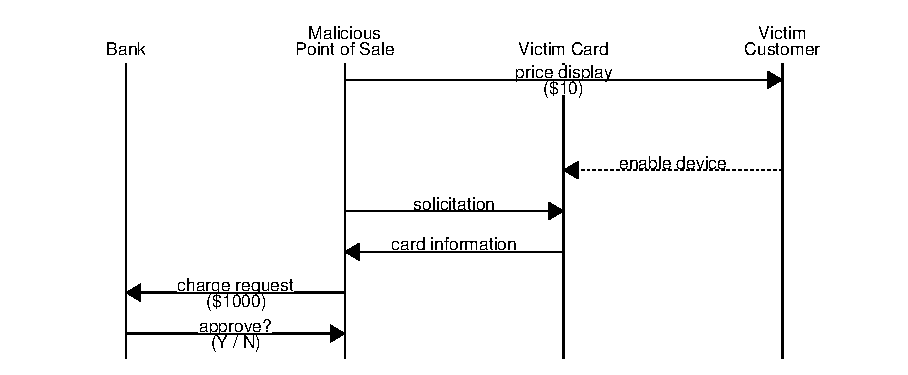
\includegraphics{img/attack-mr-overcharge.eps}
  \label{fig:attack_overcharge}
\end{figure}

Should a Customer become aware of an over-charge when reviewing his monthly statement, he may file a charge-back request with his Bank, nullifying the payment as fraudulent.
As a result, while the amount by which the Customer may be overcharged is unconstrained by the protocol, it should be relatively small for the attack to ultimately be successful.
For example, it is easy to notice a gas station charge for \$500.00 instead of \$21.87 on a monthly statement, and the resulting investigation would be uncomplicated.
However, should the struggling business choose to increase charges by 5\%, the resulting gas station charge of \$22.96 could very easily be overlooked.
Even were it to be noticed, the victim Customer may have difficulty proving the discrepancy.


\subsection{The Transparent Bridge Attack}

A more interesting attack is described by Drimer and Murdoch \cite{Drimer:2007:KYE:1362903.1362910}.
The authors consider a man-in-the-middle attack, perpetrated by a malicious Retailer and an accomplice with specialized equipment.
This attack involves four parties: a victim Customer, a malicious Retailer, a malicious Customer, and a victim Retailer.
The malicious retailer and the malicious customer collude to perform this attack.

The malicious Customer is issued with a special device, capable of relaying all messages it receives from a Point of Sale to the malicious Retailer in real time.
Similarly, it can relay any responses it receives from the malicious Retailer back to this Point of Sale.
As a result, the malicious Customer and malicious Retailer can together form a bridge between the victim Credit Card and the victim Retailer's Point of Sale.
The attack is illustrated in Figure \ref{fig:attack_bridge} and runs as follows:

\begin{enumerate}
\item First, the victim Customer attempts to make a relatively inexpensive purchase from the malicious Retailer.
Simultaneously, the malicious Customer prepares to make a relatively expensive purchase from a victim Retailer.
\item The victim Retailer's Point of Sale issues a Solicitation message to the malicious Customer, who relays it to the malicious Retailer.
\item The malicious Retailer then forwards this Solicitation message to the victim Credit Card.
\item The victim Credit Card responds with a Card Information message to the malicious Point of Sale, who relays this message to the malicious Customer.
\item The malicious Customer forwards this Card Information message to the victim Retailer's Point of Sale.
\item The victim Retailer's Point of Sale issues a Charge Request message to the victim Credit Card's bank, charging the victim Customer for the expensive purchase.
\end{enumerate}

\begin{figure}
  \caption{Transparent Bridge Attack}
  \centering
  	\hspace*{-0.35in}
    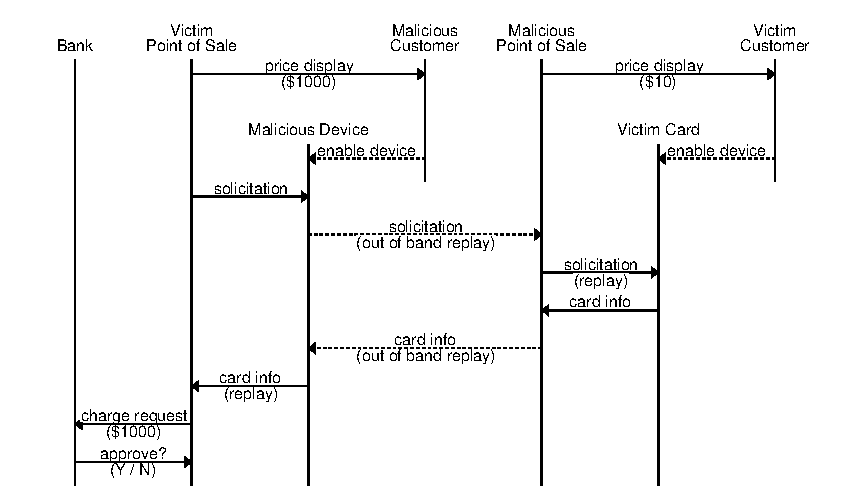
\includegraphics{img/attack-mr-bridge.eps}
  \label{fig:attack_bridge}
\end{figure}

In this attack, all messages are transparently relayed between the victim Retailer's Point of Sale and the victim Customer's Credit Card.
As a result, the victim Customer believes himself to be making an inexpensive purchase at the malicious Retailer, while he is actually making an expensive purchase at the victim Retailer.
The malicious Retailer loses the inexpensive sale, but acquires the merchandise from an expensive purchase in exchange.

This Transparent Bridge attack is particularly interesting, because the malicious parties leave no trace with either of the victims:
to the victim Customer there is only a record of an expensive purchase at the victim Retailer, and to the victim Retailer there is only the customer record of the victim Customer.
The amount which can be successfully stolen by the malicious Retailer is unconstrained, and needs not evade notice:
	if the discrepancy is noticed and the victim Customer files a charge-back request, it will be against the victim Retailer (and not the malicious Retailer).
As such, detected or not, it is one of the two victims that will be left facing the bill, making the Transparent Bridge attack significantly more dangerous than the Over-charge attack described earlier.

Drimer et al. propose a defense against this attack in the context of EMV credit cards (colloquially known as ``chip and pin'').
However, this solution is not applicable to contactless credit cards.
